\section{Benzene --- valence and low lying conduction states}
\label{sec12:benzene}

\begin{figure}[h!]
\centering
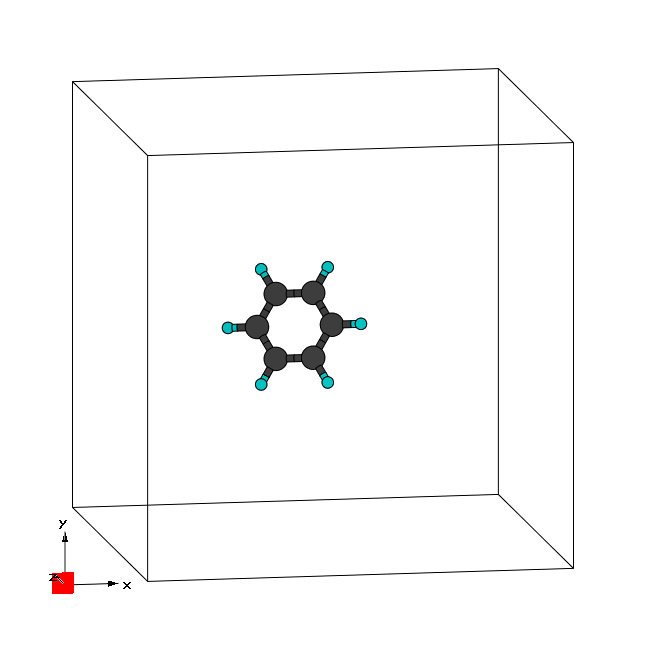
\includegraphics[width=0.25\columnwidth,trim={45pt 45pt 55pt 55pt},clip]{figure/example12/benzene.png}
\caption{Benzene molecule in periodic cell plotted with the \xcrysden{} program.}
\label{fig12.0}
\end{figure}

\subsection*{Valence States}
\begin{itemize}
\item Outline: {\it Obtain MLWFs for the valence bands of benzene.}
\end{itemize}


\begin{itemize}
\item[1-4] {\it Inspect the output file benzene.wout. The total spread converges to its minimum value after just a
few iterations.}

Convergence of total spread $\Omega$ is shown in \Fig{fig12.1}. The spread converges very quickly, and after only 15 iterations the $|\Delta\Omega|$ is already below $10^{-8}$.
Below is shown the final state of the minimization, after 22 iterations:
  \begin{tcolorbox}[sharp corners,boxrule=0.5pt]
  {\small
	\begin{verbatim}
	 Final State
  WF centre and spread    1  ( -6.875141,  7.935472,  7.937658 )     0.65233309
  WF centre and spread    2  (  4.748245,  7.935472,  7.937658 )     0.65234300
  WF centre and spread    3  (  5.809324,  6.097678,  7.937658 )     0.65186298
  WF centre and spread    4  (  7.816785, -7.396927,  7.648002 )     1.20135958
  WF centre and spread    5  (  7.816785, -7.396927, -7.648002 )     1.20135948
  WF centre and spread    6  (  7.936083,  7.324218, -7.937658 )     0.60992987
  WF centre and spread    7  (  7.935073, -6.095184,  7.937658 )     0.65161009
  WF centre and spread    8  (  6.874208, -6.712573,  7.937658 )     0.61134798
  WF centre and spread    9  (  6.874224,  6.850489, -7.648754 )     1.20500764
  WF centre and spread   10  ( -7.936214,  6.097679,  7.937658 )     0.65186256
  WF centre and spread   11  (  5.813353, -6.095183,  7.937658 )     0.65160955
  WF centre and spread   12  (  6.874224,  6.850489,  7.648754 )     1.20500766
  WF centre and spread   13  (  5.812342,  7.324217,  7.937658 )     0.60993084
  WF centre and spread   14  (  5.931632, -7.396946,  7.648001 )     1.20136423
  WF centre and spread   15  (  5.931632, -7.396946, -7.648001 )     1.20136424
  Sum of centres and spreads ( 71.362557,  7.925029, 55.563607 )    12.95829277
 
         Spreads (Ang^2)       Omega I      =    10.455434168
        ================       Omega D      =     0.000000000
                               Omega OD     =     2.502858604
    Final Spread (Ang^2)       Omega Total  =    12.958292772
 ------------------------------------------------------------------------------
	\end{verbatim}
	}
	\end{tcolorbox}

\item[5] {\it Plot the MLWFs 2-4}

MLWFs are shown in \Fig{fig12.2}.

\begin{figure}[h!]
\centering
\subfloat[Valence MLWF 2]{
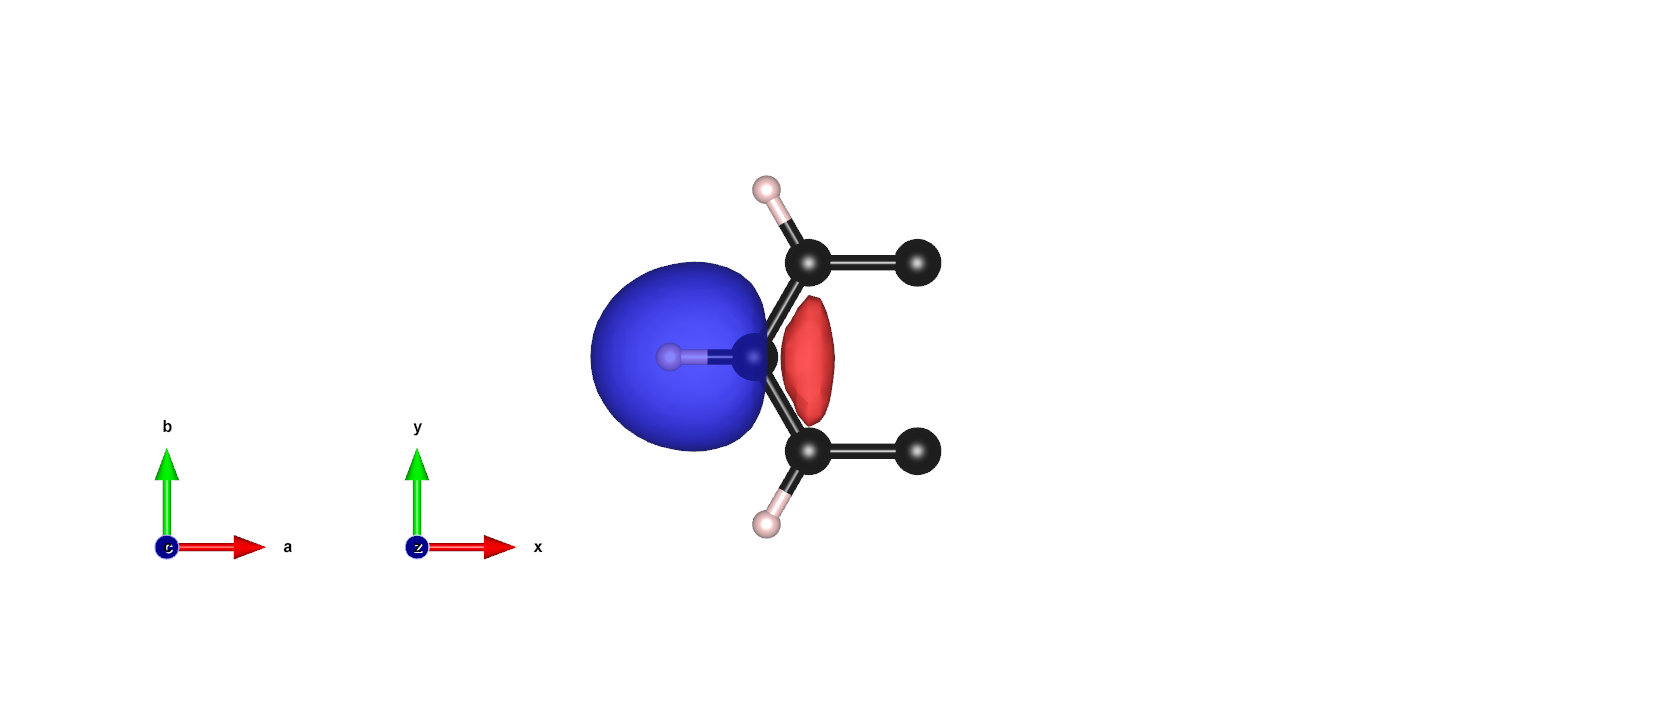
\includegraphics[width=0.3\columnwidth,trim={350pt 100pt 600pt 150pt},clip]{figure/example12/benzene_valence_2.png}}
\centering
\subfloat[Valence MLWF 3]{
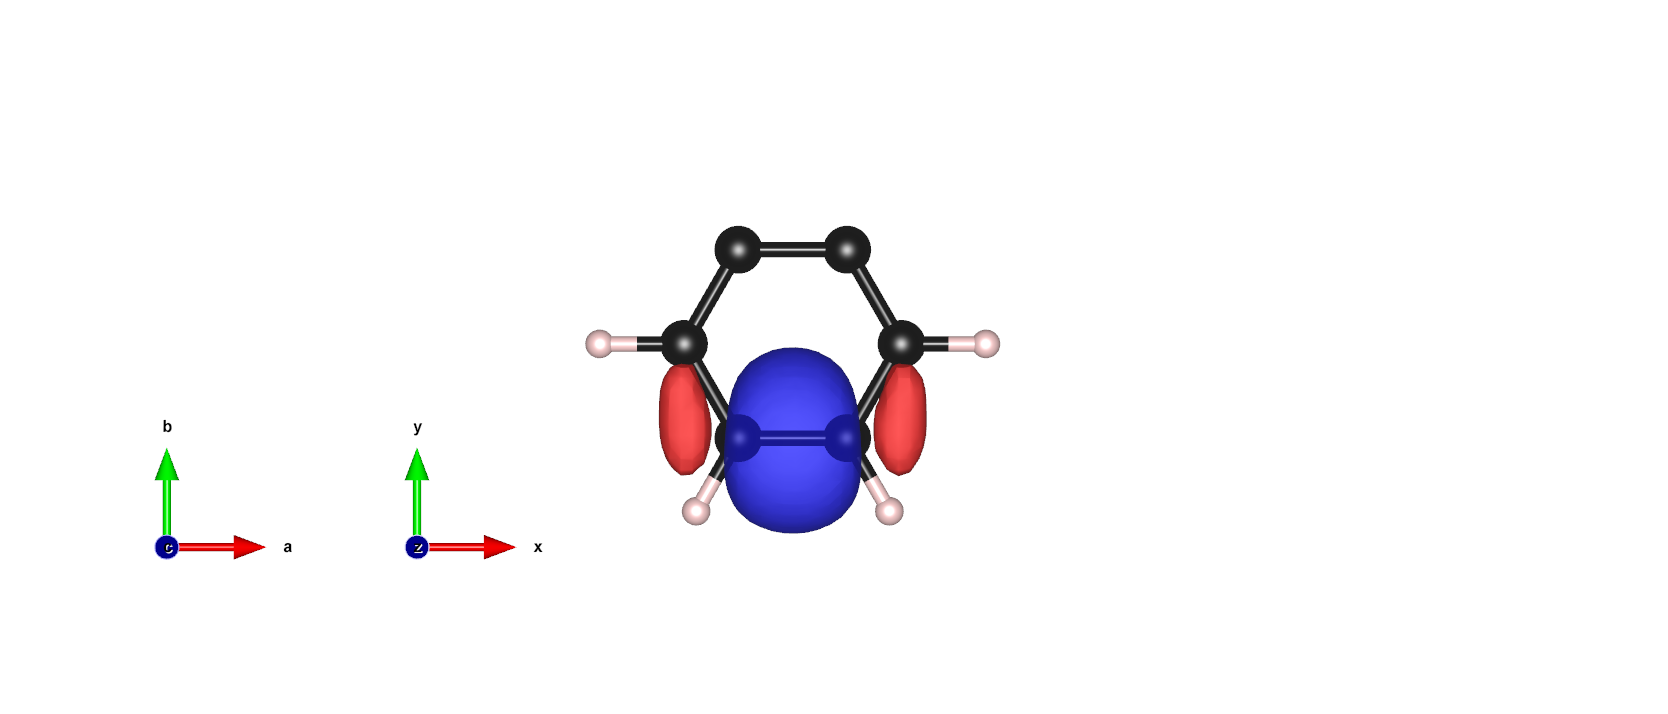
\includegraphics[width=0.3\columnwidth,trim={350pt 100pt 600pt 150pt},clip]{figure/example12/benzene_valence_3.png}}
\centering
\subfloat[Valence MLWF 4]{
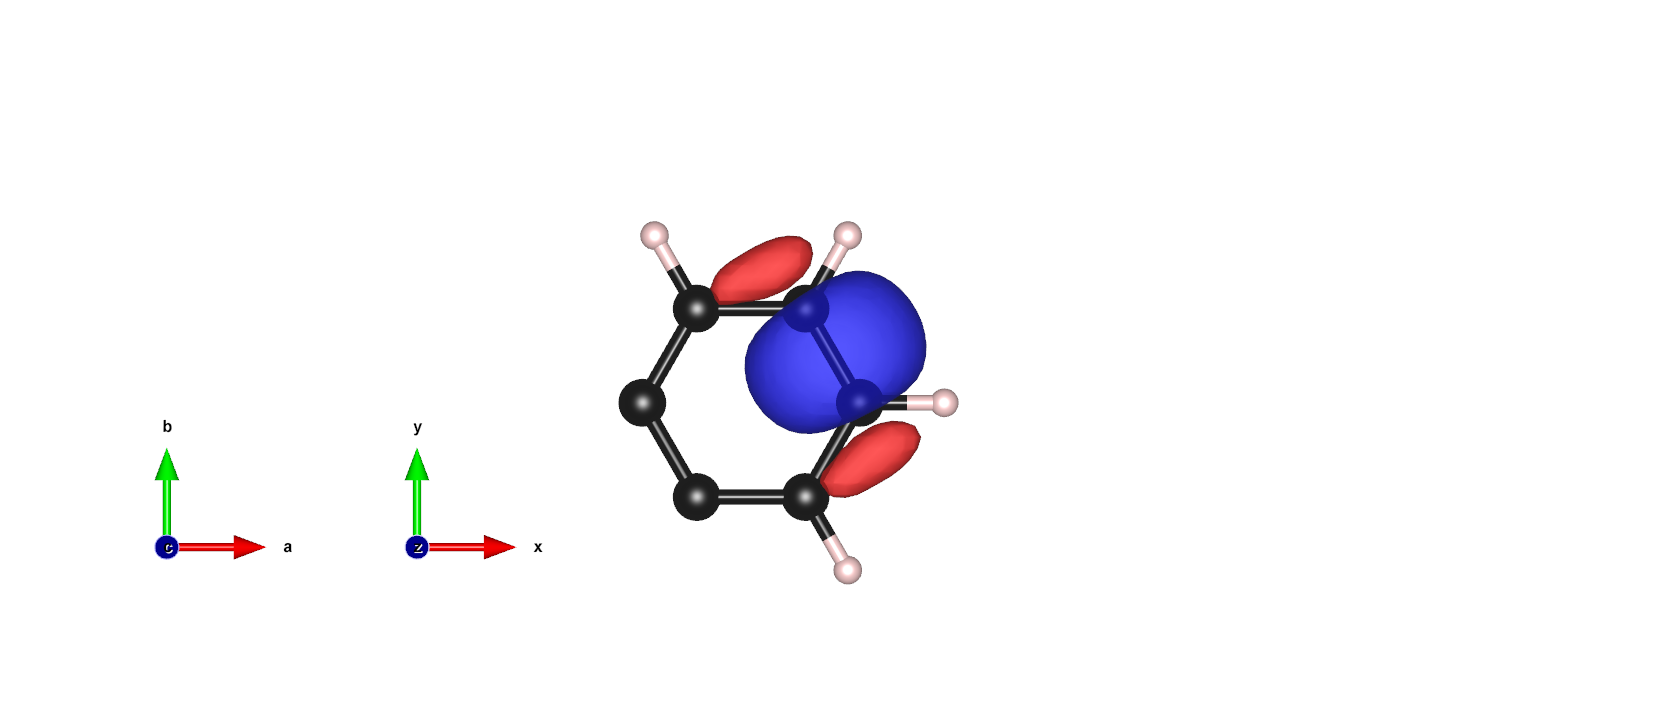
\includegraphics[width=0.3\columnwidth,trim={350pt 100pt 600pt 150pt},clip]{figure/example12/benzene_valence_4.png}}
\caption{MLWFs 2, 3 and 4, with Vesta from {\tt cube} format.}\label{fig12.2}
\end{figure}
\end{itemize}

\begin{figure}[t!]
\centering
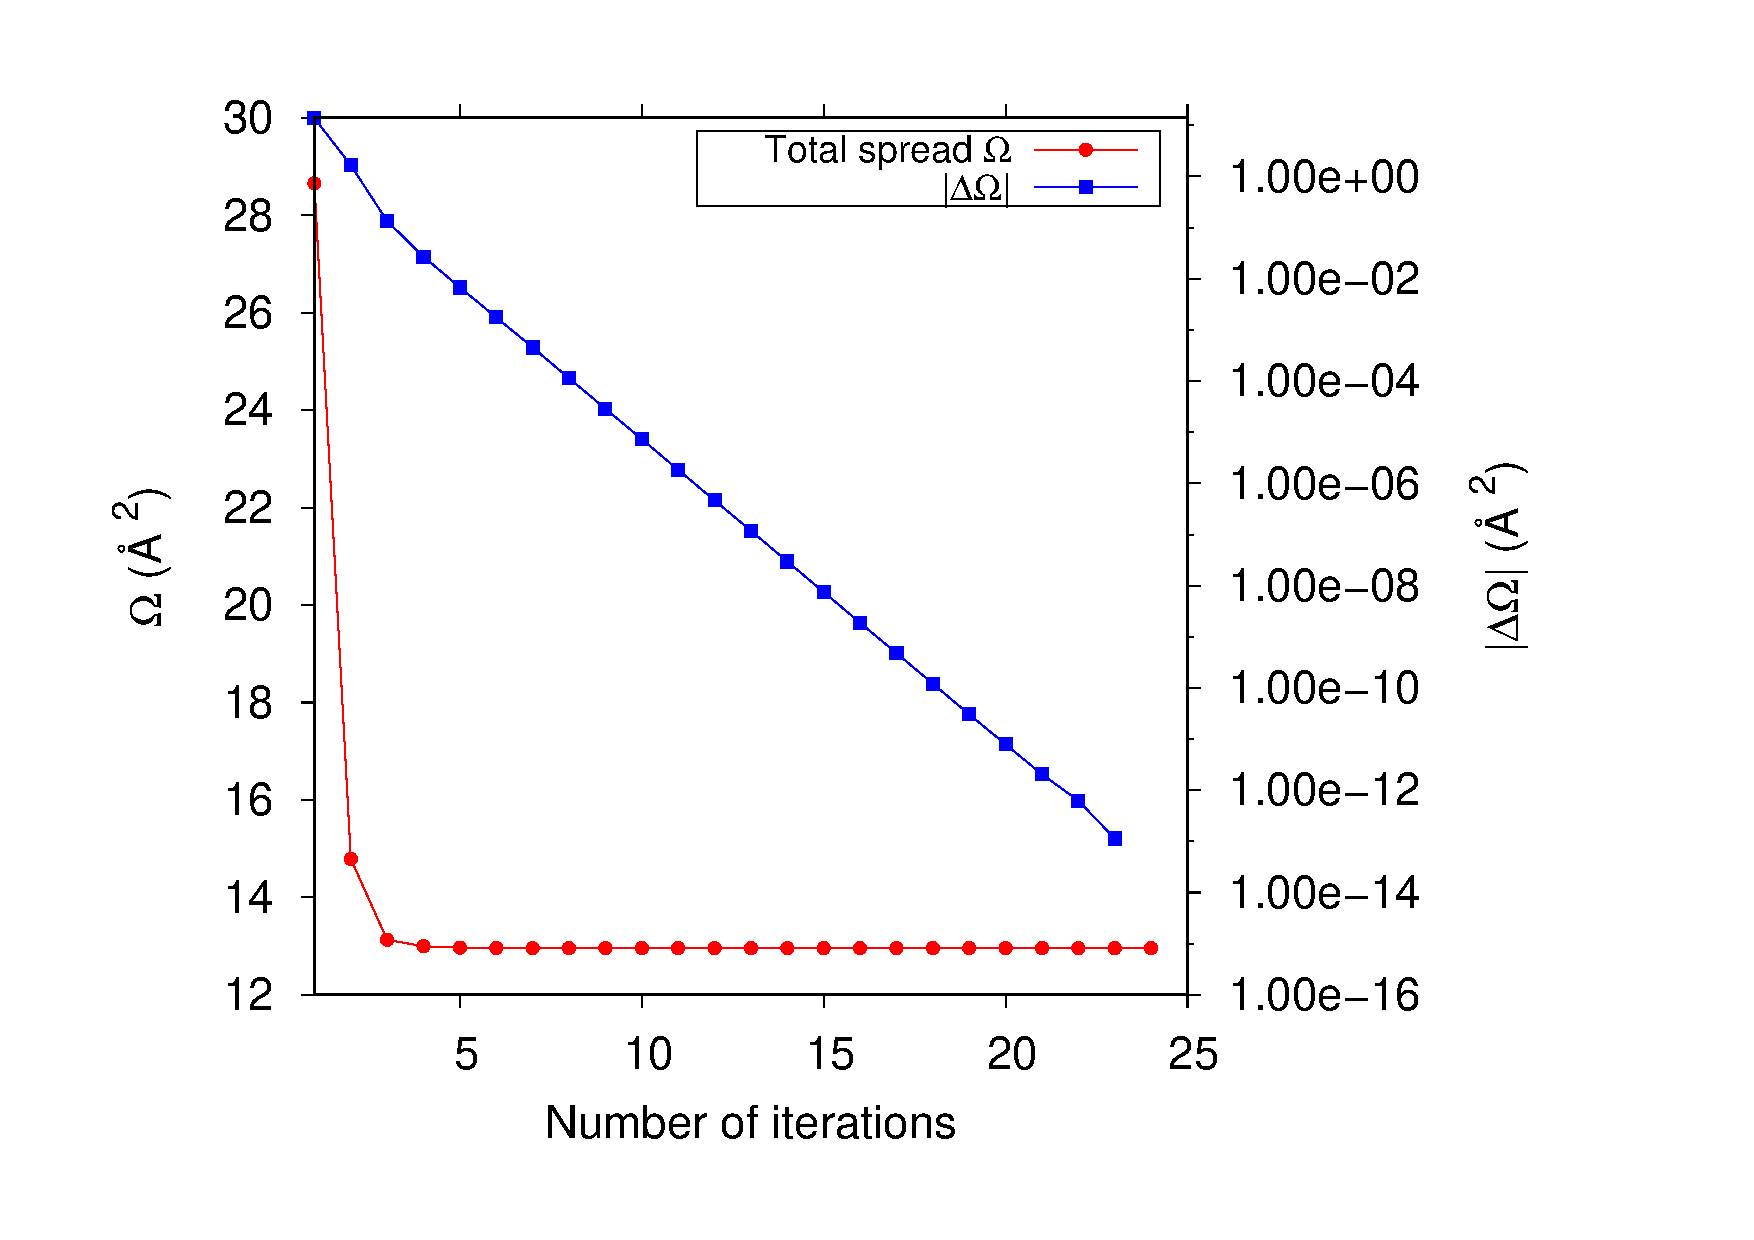
\includegraphics[width=0.7\columnwidth]{figure/example12/spread_convergence.pdf}
\caption{Convergence of total spread $\Omega$. The red curve refers to the left y-axis, i.e. the actual value of the total spread at each iteration. The blue curve refers to the right y-axis, i.e. the absolute difference between between the spread functional at iteration $i$ and $i-1$, i.e. $\Delta\Omega$.}\label{fig12.1}
\end{figure}

\subsection*{Valence + Conduction States}
\begin{itemize}
\item Outline: {\it Obtain MLWFs for the valence and low-lying conduction states of benzene.}
\end{itemize}

\begin{itemize}
\item[1] {\it First, we minimise $\Omega_I$. Then, we minimise $\Omega_D + \Omega_{OD}$.}

Extract from the {\tt .wout} output file for the disentanglement procedure with initial and final value of $\Omega_I$
  \begin{tcolorbox}[floatplacement=h!,float,nobeforeafter,sharp corners,boxrule=0.5pt]
  {\small
\begin{verbatim}
                   Extraction of optimally-connected subspace
                   ------------------------------------------
 +---------------------------------------------------------------------+<-- DIS
 |  Iter     Omega_I(i-1)      Omega_I(i)      Delta (frac.)    Time   |<-- DIS
 +---------------------------------------------------------------------+<-- DIS
       1      14.77292507      14.36793746       2.819E-02      0.06    <-- DIS
       .		.					.				.			 .
       .		.					.				.			 .
      76      14.26979011      14.26979011       7.234E-11      0.34    <-- DIS

             <<<      Delta < 1.000E-10  over  3 iterations     >>>
             <<< Disentanglement convergence criteria satisfied >>>

        Final Omega_I    14.26979011 (Ang^2)

 +----------------------------------------------------------------------------+		
\end{verbatim}
}
\end{tcolorbox}

\begin{figure}[h!]
\centering
\subfloat[Valence MLWF 1]{
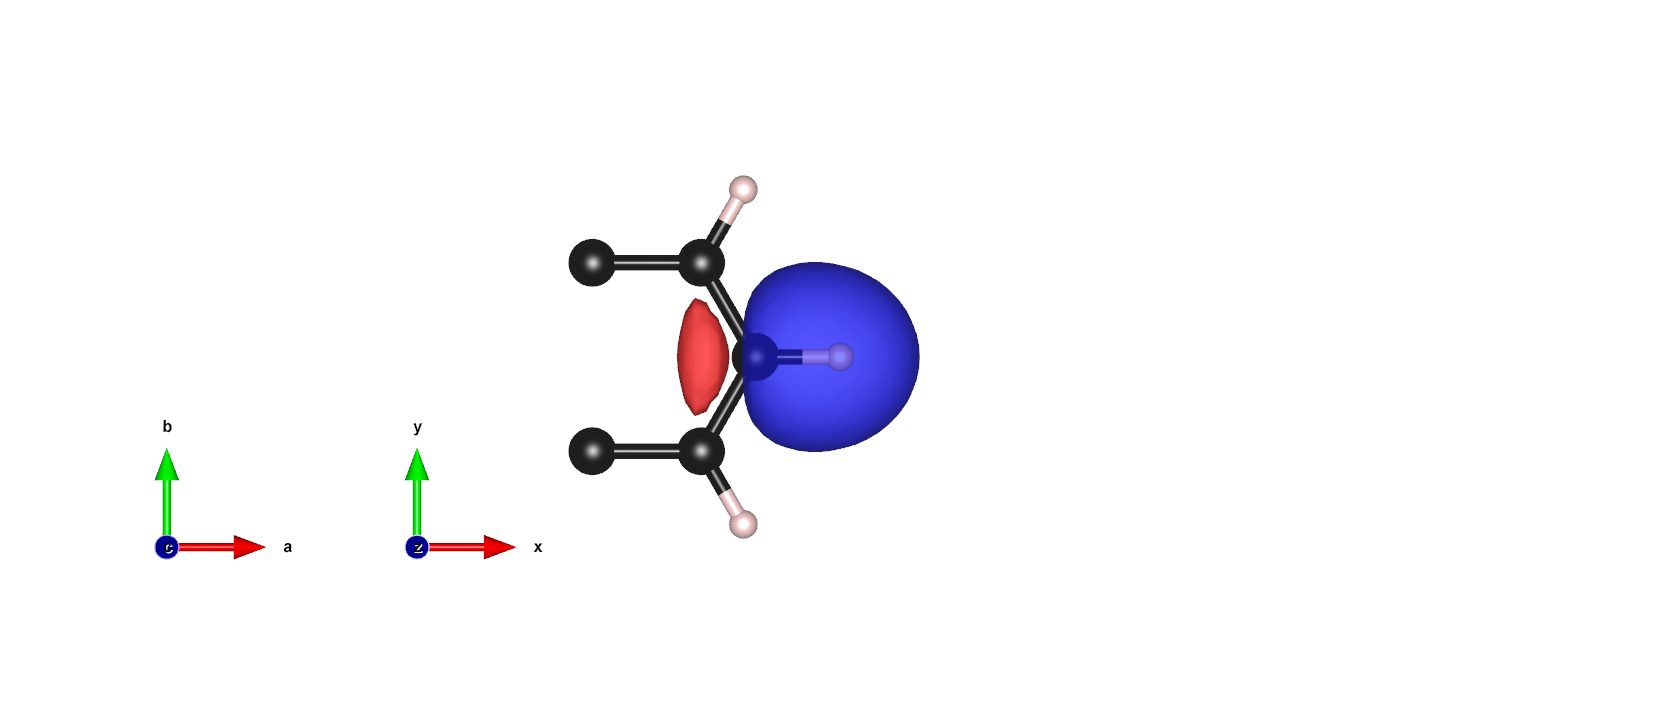
\includegraphics[width=0.3\columnwidth,trim={350pt 100pt 600pt 150pt},clip]{figure/example12/benzene_v+c_1.png}}
\centering
\subfloat[Valence MLWF 7]{
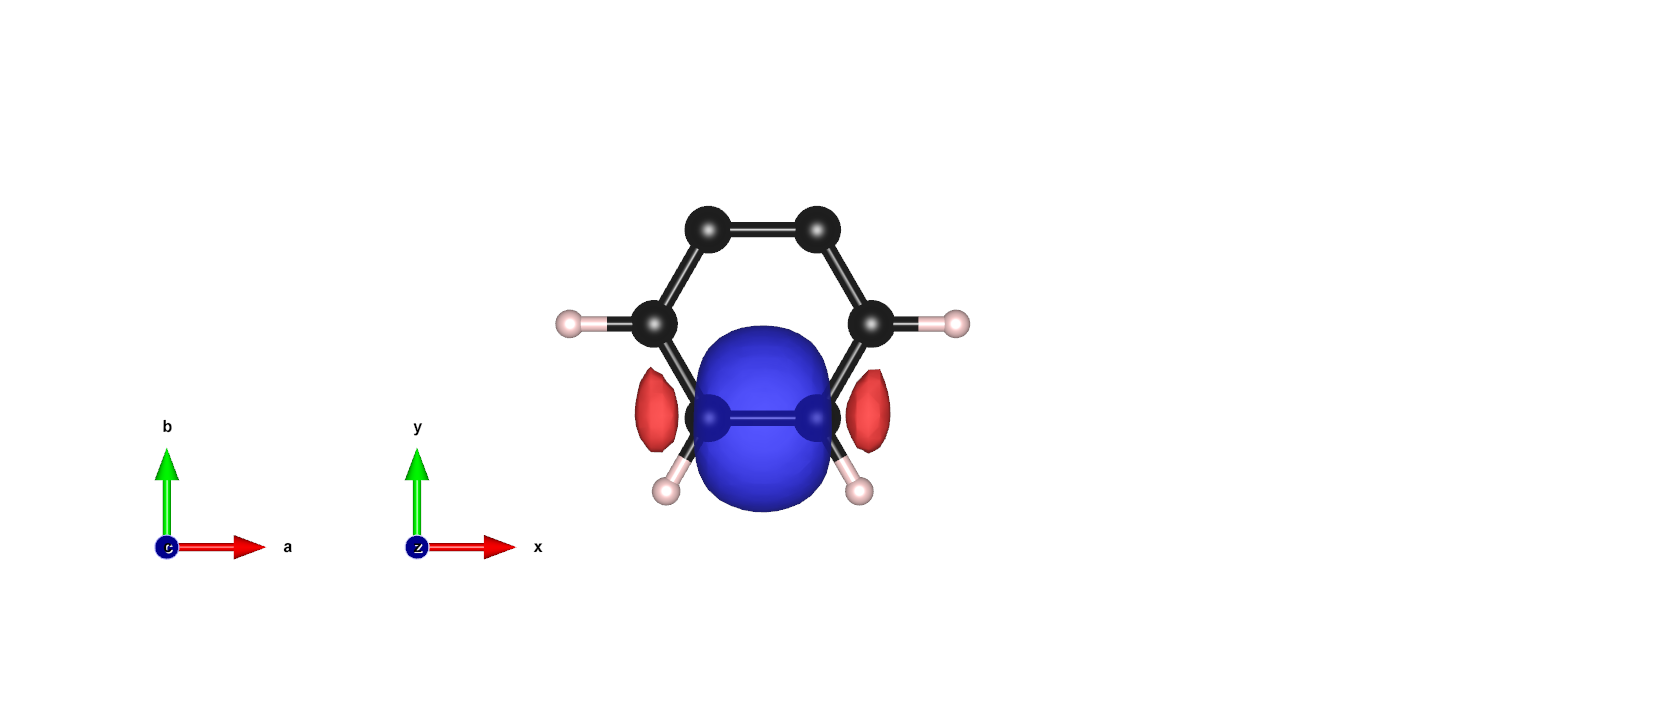
\includegraphics[width=0.3\columnwidth,trim={350pt 100pt 600pt 150pt},clip]{figure/example12/benzene_v+c_7.png}}
\centering
\subfloat[Conduction MLWF 13]{
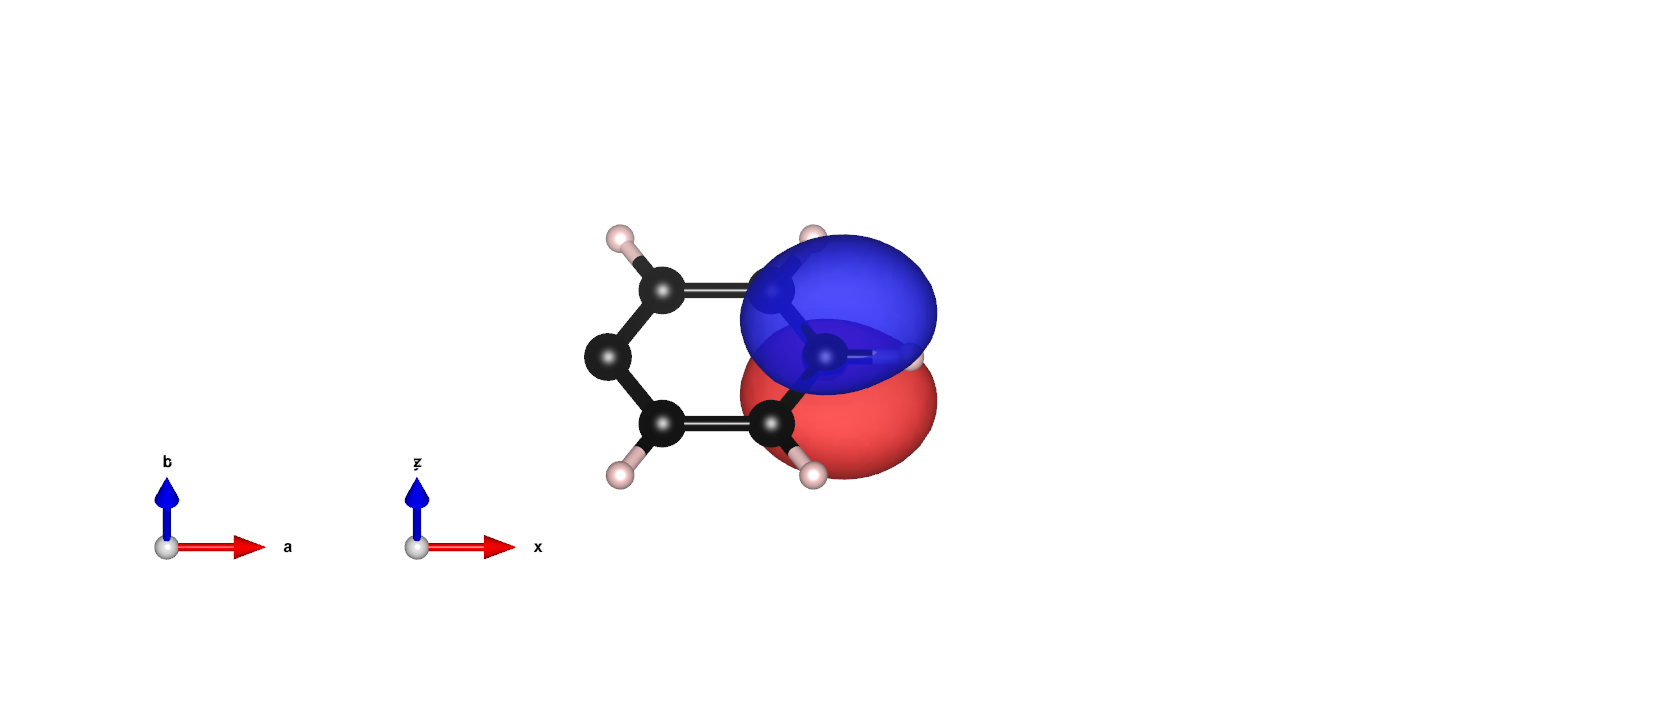
\includegraphics[width=0.3\columnwidth,trim={350pt 100pt 600pt 150pt},clip]{figure/example12/benzene_v+c_13.png}}
\caption{MLWFs 1, 3 and 13 with Vesta from {\tt cube} format.}\label{fig12.3}
\end{figure}


Below a snippet from the {\tt .wout} output file, showing the finale state of the minimisation of $\Omega_D$ and $\Omega_OD$.
  \begin{tcolorbox}[floatplacement=h!,float,nobeforeafter,sharp corners,boxrule=0.5pt]
  {\small
\begin{verbatim}
 Final State
  WF centre and spread    1  ( -6.872991, -7.937658,  7.937657 )     0.64685210
  WF centre and spread    2  ( -7.937084, -6.094542, -7.937656 )     0.64620663
  WF centre and spread    3  (  5.810194, -6.094542,  7.937654 )     0.64620672
  WF centre and spread    4  (  4.746097, -7.937658,  7.937657 )     0.64685949
  WF centre and spread    5  (  5.810193,  6.094541, -7.937657 )     0.64620720
  WF centre and spread    6  ( -7.937083,  6.094541,  7.937655 )     0.64620743
  WF centre and spread    7  (  6.874209,  6.725491,  7.937658 )     0.58709128
  WF centre and spread    8  (  6.874209, -6.725491,  7.937657 )     0.58709059
  WF centre and spread    9  (  5.824168, -7.331141,  7.937657 )     0.58581741
  WF centre and spread   10  (  5.824168,  7.331141, -7.937658 )     0.58581778
  WF centre and spread   11  (  7.924257,  7.331142,  7.937657 )     0.58581692
  WF centre and spread   12  (  7.924257, -7.331141, -7.937658 )     0.58581674
  WF centre and spread   13  ( -7.514755,  7.937658, -7.937656 )     1.57077288
  WF centre and spread   14  (  7.622957, -6.642249,  7.937655 )     1.58413409
  WF centre and spread   15  (  6.125499, -6.642276, -7.937651 )     1.58406298
  WF centre and spread   16  (  5.387848, -7.937658, -7.937656 )     1.57079972
  WF centre and spread   17  (  6.125498,  6.642275,  7.937656 )     1.58407213
  WF centre and spread   18  (  7.622957,  6.642249, -7.937653 )     1.58414266
  Sum of centres and spreads ( 60.234596,-15.875317, 15.875317 )    16.87397474

         Spreads (Ang^2)       Omega I      =    14.269790106
        ================       Omega D      =     0.000000000
                               Omega OD     =     2.604184635
    Final Spread (Ang^2)       Omega Total  =    16.873974742
 ------------------------------------------------------------------------------
\end{verbatim}
}
\end{tcolorbox}
\end{itemize}


\begin{itemize}
\item[2] {\it Plot the MLWFs 1, 7 and 13.}

MLWFs are shown in \Fig{fig12.3}.

\end{itemize}
